\section{Aufbau}
\label{sec:Aufbau}
Eine Skizze des grundlegenden Versuchaufbaus ist in Abbildung \ref{fig:aufbau}
zu sehen. Bei einseitiger Auflage wurde der Stab auf der rechten Seite (A)
mit einer Schraube (C) fixiert,
bei zweiseitiger Auflage konnte die linke Seite nur aufgelegt werden (B).
Die Schiene auf der die Messuhren befestigt sind,
ist mit einem cm-Maß beschriftet.
Die Messuhren haben eine kleine Anzeige zur Represäntation der mm.
Die große Skala ist in 10 0,1mm Stücke unterteilt,
welche ebenfalls in 10 Teilstücke unterteilt sind.
Die Messung bei einseitiger Auflage erfolgte mit einer Messuhr.
Der jeweilige Stab ragte 50cm weit in den Bereich der Messuhren hinein.
Das Gewicht wurde am freien Ende des Stabes eingehängt.
Bei beidseitiger Auflage hing das Gewicht in der Mitte des Stabes
und es wurde mit beiden Messuhren gemessen.

\begin{figure}
  \centering
  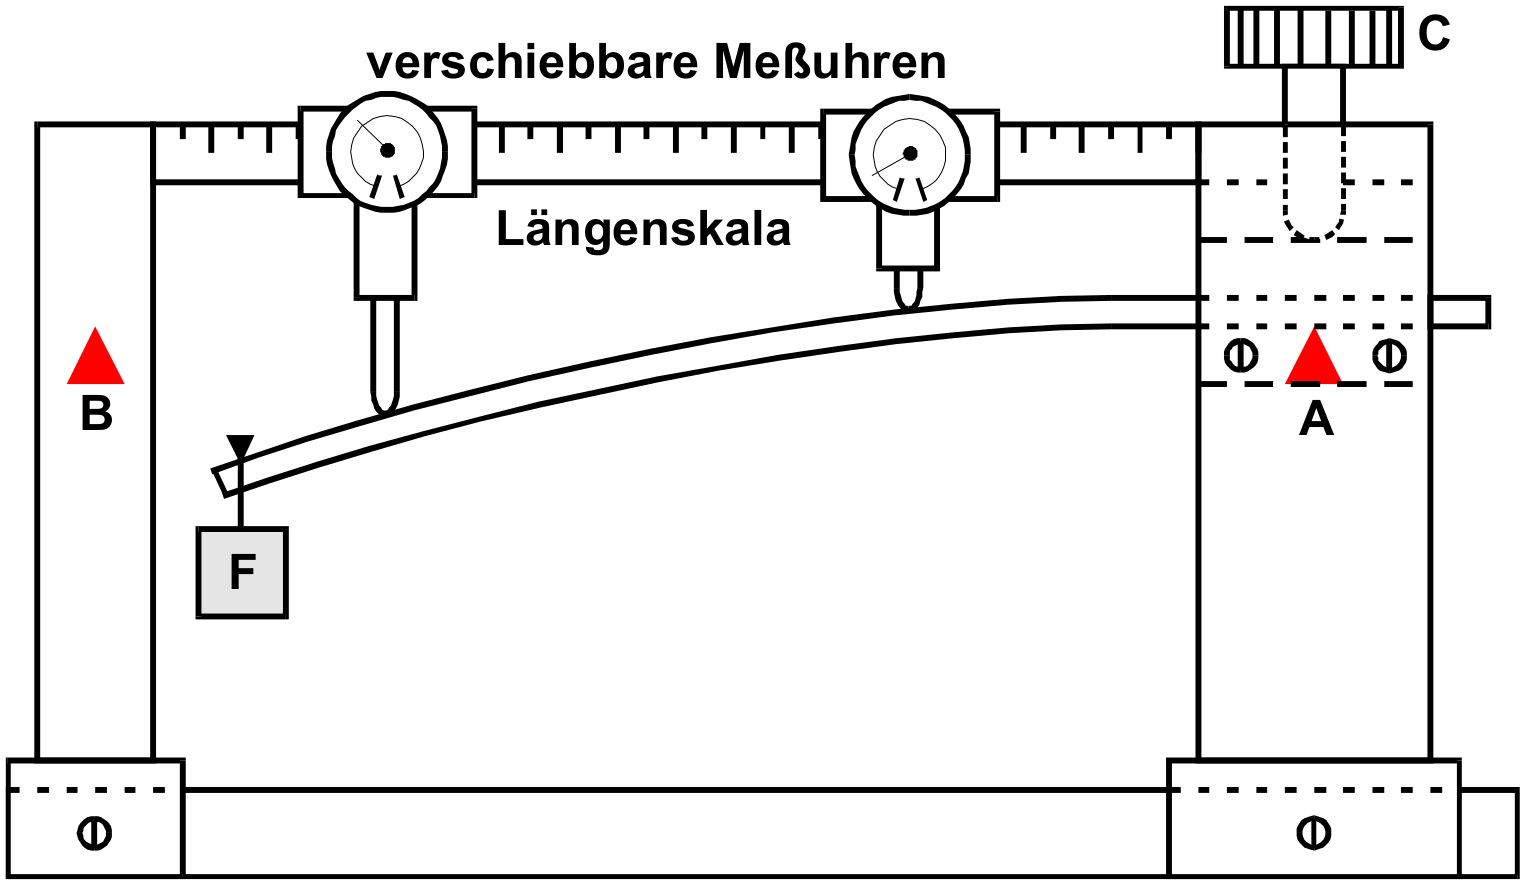
\includegraphics[width=\textwidth]{content/aufbau.jpg}
  \caption{Schematische Darstellung des Versuchsaufbaus. \cite{Anleitung}}
  \label{fig:aufbau}
\end{figure}
